\documentclass[12pt]{article}
\usepackage[utf8]{inputenc}
\usepackage{amsmath, amssymb}
\usepackage{hyperref}
\usepackage{tikz}
\usepackage[left=2.5cm,right=2.5cm,bottom=2.5cm]{geometry}

\hypersetup{
    colorlinks=true}

\title{MATH 5707 (Spring 2026): Homework 2}
\date{}

\begin{document}
\vspace{-0.7in}

\maketitle
\vspace{-0.6in}

\section*{Directions and Introduction}
Submit a pdf of your solutions to the HW 2 assignment on Gradescope by 11:59 pm on February 13.

Problem 4 is marked as a peer review problem. \href{https://docs.google.com/document/d/1jSw9pmMJJFUx_6dTkcUi4k4HJNIrrIIgs9zdWhAycx0/edit?usp=sharing}{This document gives directions and deadlines for the peer review process.}

When working on this assignment, you should focus on the following goals:
\begin{itemize}
    \item Clearly communicate solutions using complete sentences and enough explanation that another 5707 student could follow your work.
    \item Demonstrate fluency with the concepts of Eulerian and Hamiltonian graphs.
    \item Translate a scenario or problem into a question or statement about graphs.
    \item Demonstrate fluency with basic graph theory terminology and notation, such as $\nu(G)$, $\varepsilon(G)$, bipartite, complete, simple graph, multigraph, cycles, etc.
    \item Demonstrate fluency with basic graph theory operations.
    \item Given a set of properties, draw a graph that satisfies those properties or explain why no such graph can exist.
    \item When given a new graph theoretic definition, prove something about it.
\end{itemize}


\section*{Problems}

\begin{enumerate}
    \item Draw a graph $G$ that satisfies the following properties, or explain why one does not exist.
    \begin{itemize}
        \item $G$ is not Eulerian.
        \item $G$ is Hamiltonian.
        \item $\nu(G)=6$
        \item $\varepsilon(G)=10$
    \end{itemize}
\newpage
    \item  Describe each graph below using basic graph families and graph operations.  (The graph operations to consider are complements, disjoint unions, joins, and Cartesian products.)

    \vspace{-.1in}
    \begin{center}
    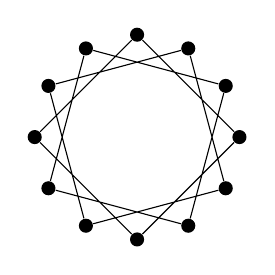
\begin{tikzpicture}
    \draw[every node/.style={inner sep=1.8pt,fill,circle}]
    (0,0) \foreach \y in {0,1,2,3}{ 
    \foreach \x in {0,1,2}{
    +(90+30*\x+90*\y:1.3)node(x\x\y){} }}
    (x00)--(x01)--(x02)--(x03)--(x00)
    (x10)--(x11)--(x12)--(x13)--(x10)
    (x20)--(x21)--(x22)--(x23)--(x20);
    \end{tikzpicture}
    \hspace{1in}
    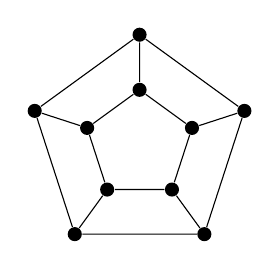
\begin{tikzpicture}
    \draw[every node/.style={inner sep=1.8pt,fill,circle}]
    (0,0) \foreach \y in {0,1,2,3,4}{ 
    \foreach \x in {0,1}{
    +(90+72*\y:.7+.7*\x)node(x\x\y){} }}
    (x00)--(x01)--(x02)--(x03)--(x04)--(x00)
    (x10)--(x11)--(x12)--(x13)--(x14)--(x10)
    (x00)--(x10) (x01)--(x11) (x02)--(x12) (x03)--(x13) (x04)--(x14);
    \end{tikzpicture}
    \hspace{1in}
    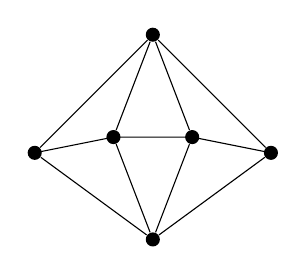
\begin{tikzpicture}
    \draw[every node/.style={inner sep=1.8pt,fill,circle}]
    (-1.5,-.2)node(x1){}--(-.5,0)node(x2){}--(.5,0)node(x3){}--(1.5,-.2)node(x4){};
    \draw[every node/.style={inner sep=1.8pt,fill,circle}]
    (0,1.3)node(a){} (0,-1.3)node(b){}
    \foreach \x in {1,2,3,4}{
    (a)--(x\x)--(b)};
    \end{tikzpicture}
    \end{center}

    \item Let $G_1$ and $G_2$ be two Eulerian graphs with no vertex in common. Let $v_1$ be a vertex in $G_1$ and let $v_2$ be a vertex in $G_2$. Let $G$ be the graph obtained from $G_1 \cup G_2$ by adding the edge $v_1v_2$.
    \begin{enumerate}
        \item Does $G$ have an Eulerian circuit? Explain why or why not.
        \item Does $G$ have an Eulerian trail? Explain why or why not.
    \end{enumerate}

    \item (Peer Review Problem; 4.2.2 from Bondy-Murty) A mouse eats his way through a $3 \times 3 \times 3$ cube of cheese by tunneling through all of the 27 $1 \times 1 \times 1$ subcubes. If he starts at one corner and always moves on to an uneaten subcube, can he finish at the center of the cube?

    \item (4.2.11(a) from Bondy-Murty) We say that $G$ is \textit{Hamilton-connected} if every two vertices of $G$ are connected by a Hamilton path. Show that if $G$ is Hamilton-connected and $\nu \ge 4$, then $\varepsilon \ge \frac{1}{2}(3\nu+1)$.
\end{enumerate}

\end{document}
